查看本节演示代码：\href{https://gitee.com/mindspore/mindquantum/blob/research/paper_with_code/variational_quantum_circuits_enhanced_generative_adversarial_network/QGAN.py}{\color{ceruleanblue}{Gitee}} \ \href{https://github.com/donghufeng/mindquantum_tutorial_code/blob/master/whitepaper/code/chapt05/5.7_Q-GAN/QGAN.py}{\color{ceruleanblue}{GitHub}}

\subsubsection{背景}
生成对抗网络（Generative Adversarial Network, GAN）是 Goodfellow 提出的一类著名机器学习模型。它在多种具有挑战性的任务中表现突出，尤其适用于图像生成和视频生成。一般的 GAN 由生成器 ${G}$ 和判别器 ${D}$ 组成，并通过 ${G}$ 与 ${D}$ 之间的对抗博弈完成生成任务。在训练过程中，${G}$ 的目标是最大化 ${D}$ 将生成数据误判为真实数据的概率；相应地，${D}$ 的目标是最大化其正确识别真实数据的概率，同时最小化其将生成数据误判为真实数据的概率。GAN 的目标函数可概括为
\begin{equation}
  \begin{split}
    \mathop {\min }\limits_G \mathop {\max }\limits_D V(D,G) = {\rm{ }}{{\rm{E}}_{x\sim{p_r}(x)}}[\log D(x)]
    \\+ {{\rm{E}}_{z\sim{p_z}(z)}}[\log (1 - D(G(z)))]. \label{eq1}
  \end{split}
\end{equation}

QGAN 作为 GAN 的量子版本，在采样和生成离散数据方面比经典对应模型具有更多优势。此外，理论上已经证明其具备潜在的指数加速能力 \cite{lloyd2018quantum}。这些优势推动了围绕 QGAN 的大量研究，例如经典或量子数据学习 \cite{benedetti2019adversarial, zeng2019learning, zoufal2019quantum,ahmed2021quantum}、利用量子线路纠缠能力克服非凸性和模式崩塌问题 \cite{niu2022entangling}、小分子药物发现 \cite{li2021quantum}、数据增强 \cite{nakaji2021quantum}，以及基于 QGAN 的异常检测 \cite{herr2021anomaly}。

\subsubsection{实现}
本节展示如何使用 \MindQuantum\ 构建一个混合量子-经典生成对抗网络（QC-GAN）\cite{shu2024variational}，并通过训练学习一个概率分布，从而生成手写数字。具体而言，QC-GAN 使用一个变分量子线路和一层神经网络组成 ${G}$，并使用经典神经网络组成 ${D}$。其训练方式与经典 GAN 类似：将噪声向量 ${z}$ 输入 ${G}$，随后通过 ${G}$ 和 ${D}$ 的对抗训练实现图像生成。
不同之处在于，生成图像由量子线路演化、测量以及神经网络的非线性映射共同得到。QC-GAN 的整体结构和训练过程如图 \ref{qc-gan} 所示。

\begin{figure}[ht]
  \centering
  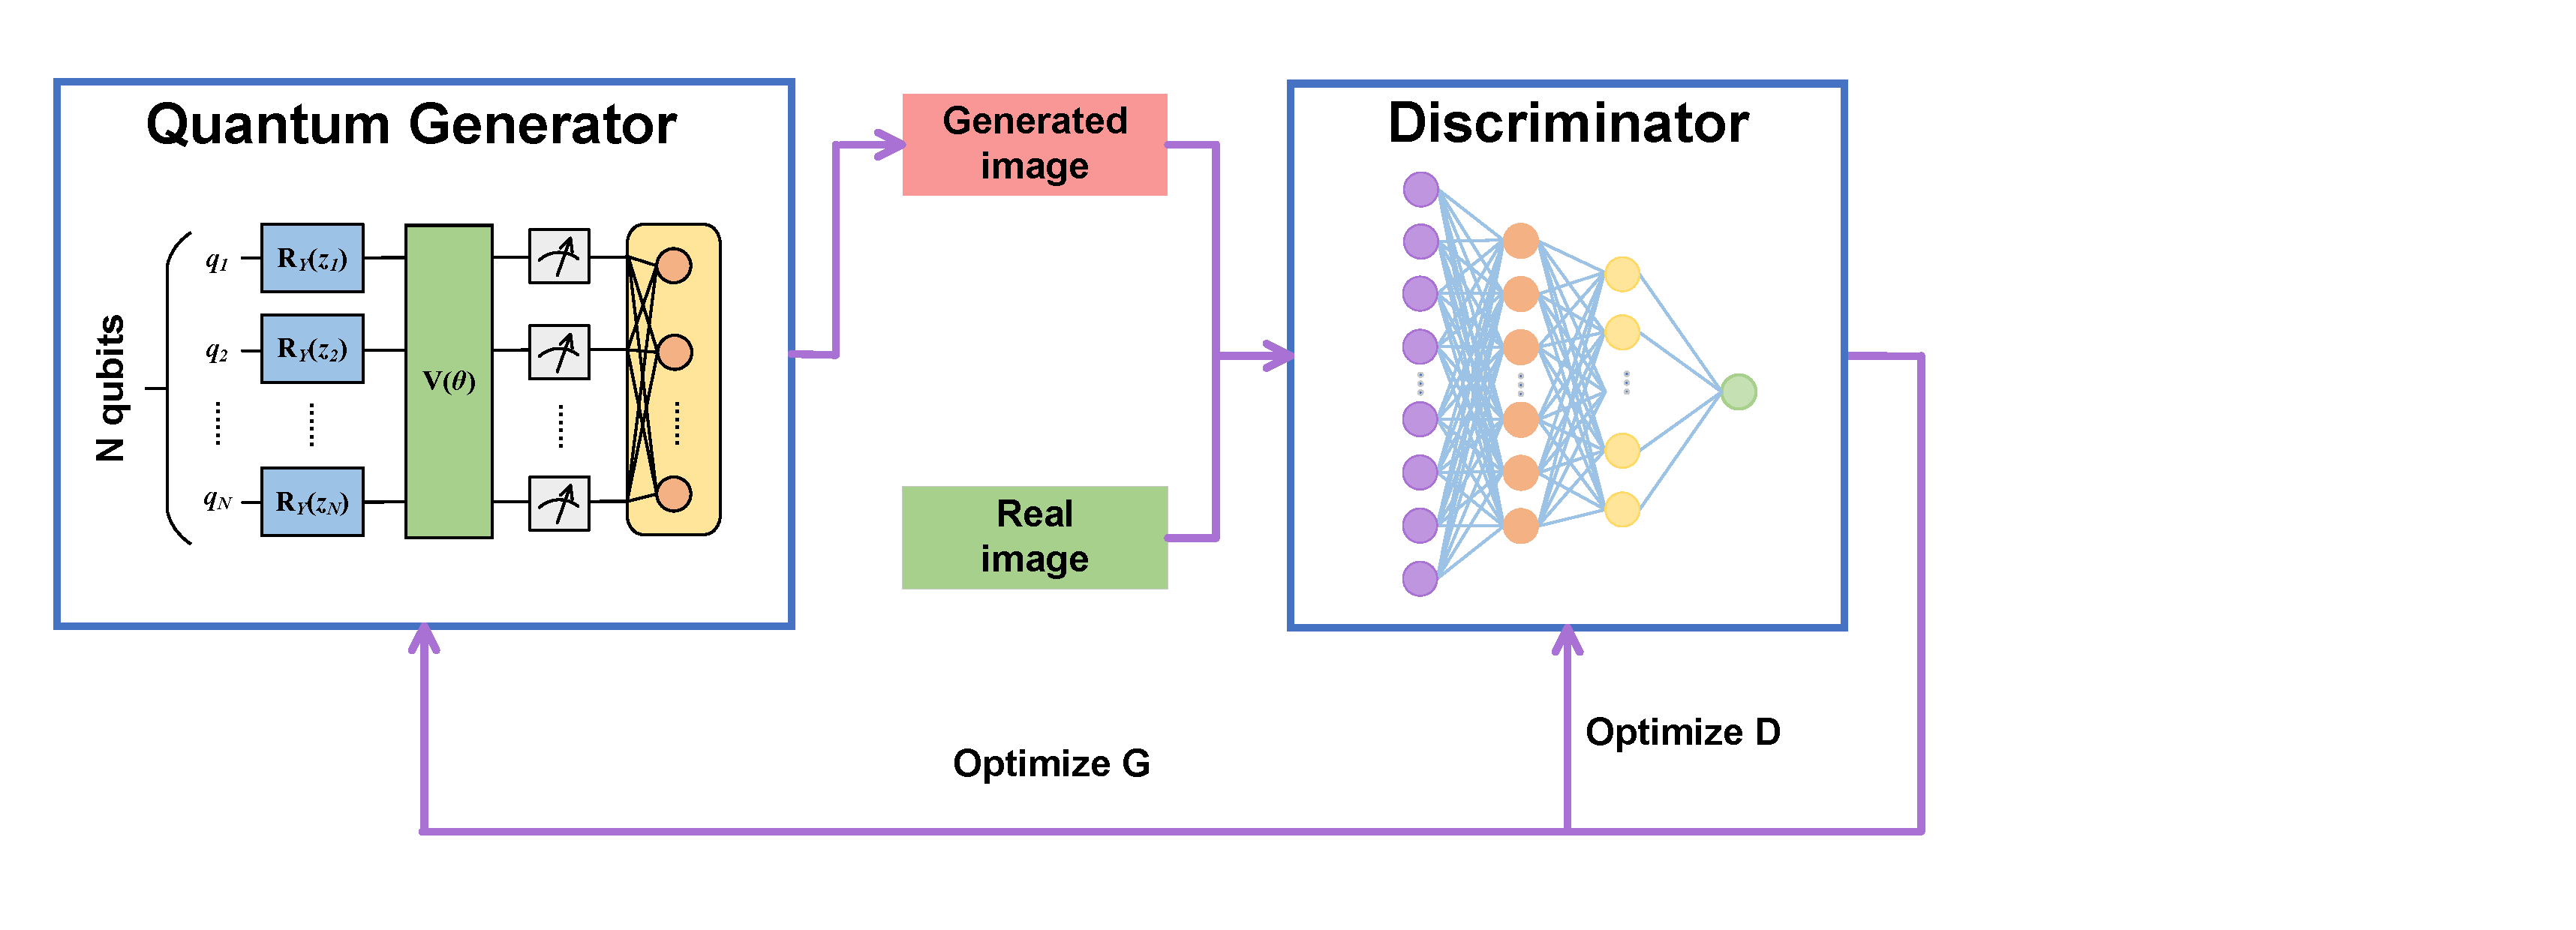
\includegraphics[scale=0.2]{5.4.4_figures/qc-gan.pdf}
  \caption{\label{qc-gan} QC-GAN 的整体架构与训练过程。}
\end{figure}

第一步是加载数据集。实验使用手写数字数据集，该数据集共有 70,000 张手写数字图像，其中包含 60,000 个训练样本和 10,000 个测试样本；图像尺寸为 28*28，且为单通道图像。加载数据集后，需要执行一系列预处理操作，为后续训练做准备。模型构建部分由两个网络组成，即生成器 ${G}$ 和判别器 ${D}$。判别器部分采用常规全连接网络结构。生成器则分为量子部分和经典部分。量子线路通过调用 \MindQuantum\ 的参数化旋转门构建，具体如下。量子线路结构可以通过 \Circuit\ 的 \methodsummary 方法展示。
\begin{figure*}[htbp]
  \centering
  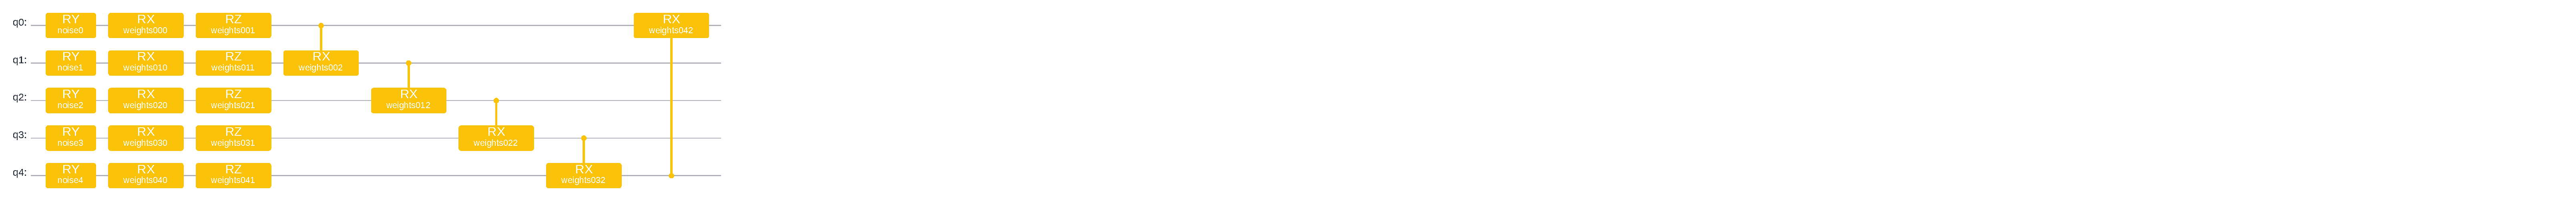
\includegraphics[scale=0.5]{5.4.4_figures/circuit.pdf}
  \caption{\label{quantum-circuit} 量子线路。}
\end{figure*}

\begin{lstlisting}
def quantum_circuit():
  encoder = Circuit()
  for i in range(qubits):
      encoder += RY(f'noise{i}').on(i)
  encoder = encoder.no_grad()
  ansatz = Circuit()
  for i in range(depth):
      for k in range(gate):
          for j in range(qubits):
              if k == 0:
                  ansatz += RX(f'weights{i}{j}{k}').on(j)
              elif k == 1:
                  ansatz += RZ(f'weights{i}{j}{k}').on(j)
              elif k == 2:
                  if j < 4:
                      ansatz += RX(f'weights{i}{j}{k}').on(j + 1, j)
                  else:
                      ansatz += RX(f'weights{i}{j}{k}').on(0, j)
  circuit = encoder.as_encoder() + ansatz.as_ansatz()
  return circuit
\end{lstlisting}
将量子线路按层堆叠并测量输出，即可构成一个量子层。
\begin{lstlisting}
def quantum_layer(qubits):
    circuit = quantum_circuit()
    circ_l = Circuit()
    hams = quantum_measure(qubits)
    sim = Simulator('mqvector', circuit.n_qubits)
    sim_l = Simulator('mqvector', qubits)
    grad_ops = sim.get_expectation_with_grad(hams, circuit, circ_l, sim_l, parallel_worker=4)

    QuantumNet = MQLayer(grad_ops,
                         weight=ms.Tensor(np.random.uniform(-np.pi, np.pi, len(circuit.ansatz_params_name)),
                         dtype=ms.dtype.float32))
    return QuantumNet
\end{lstlisting}

随后，与构建经典神经网络类似，定义网络的各个层并设置前向传播过程，即可组成量子生成器模型。反向传播过程会自动求导并更新参数。
\begin{lstlisting}
  class QuantumGenerator(nn.Cell):
    def __init__(self):
        super(QuantumGenerator, self).__init__()
        self.quantumlayer = quantum_layer(qubits)
        self.linear = nn.Dense(2**qubits, img_size * img_size, weight_init='uniform')
        self.relu = nn.ReLU()
        self.sigmoid = nn.Sigmoid()
        self.tanh = nn.Tanh()

    def construct(self, x):
        x = self.quantumlayer(x)
        x = x/(abs(x).max())
        x = self.linear(x)
        out = self.sigmoid(x)
        return out
\end{lstlisting}

量子线路参数会依据所设计的代价函数进行优化。生成器需要生成尽可能接近真实样本的概率分布，判别器则需要尽可能区分真实分布与生成分布。二者的代价函数分别设计如下。
\begin{equation}
  {L_G} =  - {{\rm E}_{x\sim{p_f}(x)}}\left[ {\log D(x)} \right],
\end{equation}
\begin{equation}
  {L_D} =  - {{\rm E}_{x\sim{p_r}(x)}}\left[ {\log D(x)} \right] - {{\rm E}_{x\sim{p_f}(x)}}\left[ {\log D(x)} \right].
\end{equation}

根据设计好的损失函数和模型，生成器与判别器会交替训练并更新参数。训练完成后，将噪声向量作为生成器输入，即可输出生成的手写数字，结果如图 \ref{qgan-result} 所示。可以看到，随着迭代次数增加，输入噪声逐渐能够生成清晰的数字图像。需要注意的是，训练迭代次数必须谨慎设计，并非越多越好。
\begin{figure}[htbp]
  \centering
  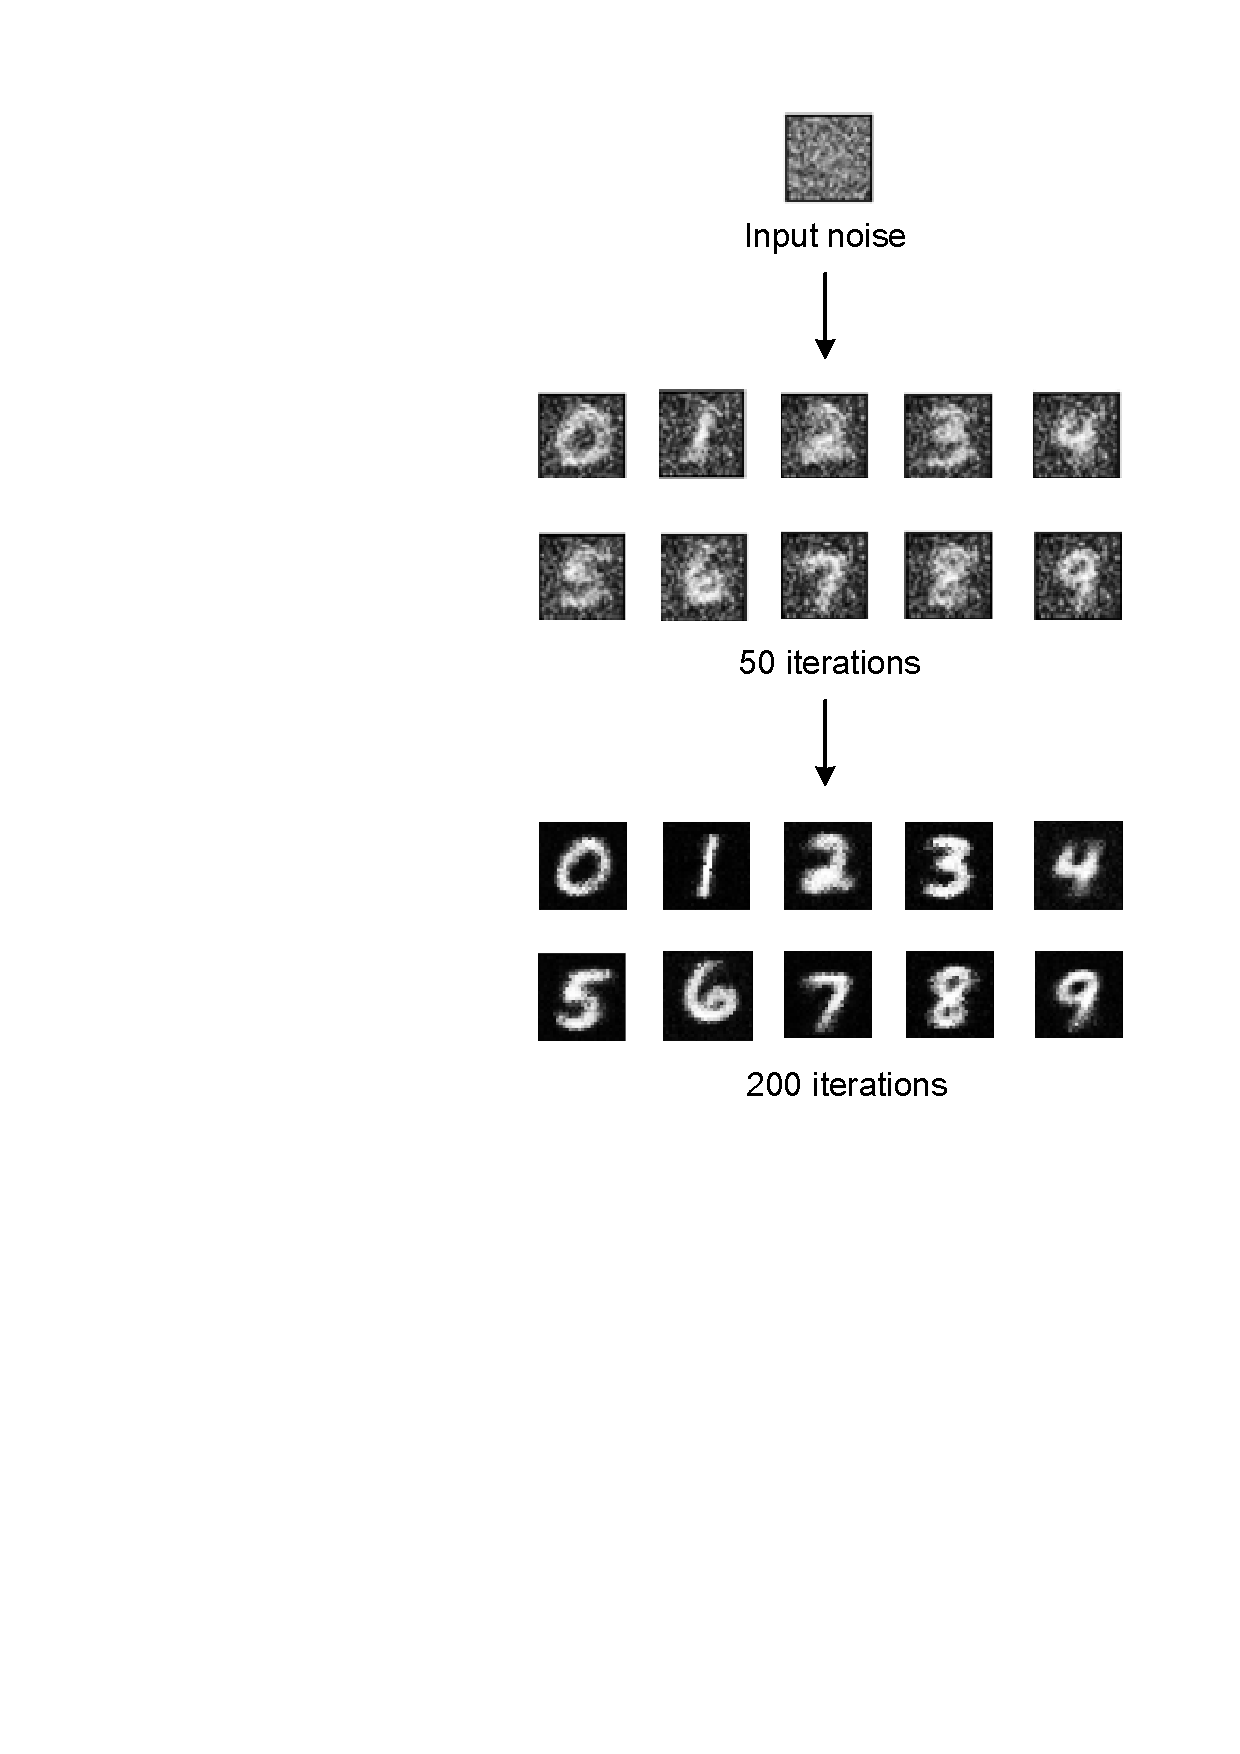
\includegraphics[scale=0.5]{5.4.4_figures/qgan-result.pdf}
  \caption{\label{qgan-result} QC-GAN 在不同训练阶段生成的手写数字结果。}
\end{figure}
